\documentclass[sigconf]{acmart}
% Formatting from the competition's supplied Overleaf template.
\setcopyright{none}
\settopmatter{printacmref=false}
\acmConference[Kaggle Competition]{Filament Segmentation Challenge}{2026}{\href{https://www.kaggle.com/competitions/filament-segmentation-2026}{kaggle.com/competitions/filament-segmentation-2026}}
\acmBooktitle{Competition Report}
\acmDOI{}
\acmISBN{}
\usepackage{xcolor}
\newif\ifguideStyle
\guideStyletrue
\newcommand{\guide}[1]{\ifguideStyle{\color{gray!65}\itshape #1}\fi}
\usepackage{mathtools}
\usepackage{subcaption}
\usepackage{tabularx}
\usepackage{multirow}

\guideStylefalse
\begin{document}
\title{Selecting Filaments by Their Expected Matched IoU}
\subtitle{A Solution to the Solar Filament Segmentation Challenge 2026}
\author{{\O}yvind Andre Roth}

\begin{abstract}
We segment solar filaments in GONG H$\alpha$ full-disk images as instances and optimise the competition metric directly. Panoptic Quality pooled over (annotator, image) pairs has a denominator that does not depend on which predictions match, so every predicted filament contributes on its own and is worth keeping exactly when its expected matched IoU exceeds PQ/2. Soft-label U-Nets estimate the probability that an annotator marks a pixel; candidate filaments are the nodes of a 15-level component tree of that map; a gradient-boosted hurdle model estimates each candidate's expected matched IoU; and a tree dynamic program selects the best non-overlapping set exactly. An optional crop refiner re-segments the selected filaments. On five date-grouped folds covering all 707 training images, out-of-fold PQ is 0.434 (0.438 with the refiner), against 0.414 for connected components at a fixed threshold chosen on validation data and 0.340 for one annotator scored against the others. The public leaderboard score is 0.37; we show that this gap is not sampling noise, input shift or an optimistic threshold.
\end{abstract}
\keywords{solar filaments, H-alpha, instance segmentation, panoptic quality, component tree}
\maketitle

\section{Introduction}
This report goes over the details of our submitted solution to the Solar Filament Segmentation Challenge~2026 \cite{filament-segmentation-2026}. The challenge, launched on July~10,~2026, is organized by the Earth-Space AI Research (ESAIR) Lab\footnote{\href{https://www.esairlab.com/home}{www.esairlab.com/}}. This challenge utilizes the MAGFiLO dataset for evaluation of the segmentation algorithms \cite{ahmadzadeh2024dataset}.

Our solution treats the metric, Panoptic Quality (PQ)~\cite{kirillov2019panoptic} pooled over annotator--image pairs, as the design specification. Section~\ref{sec:methodology} shows that pooled PQ splits into independent per-instance terms, which turns post-processing into an exact optimisation over a tree of candidate filaments. Section~\ref{sec:evaluation} reports out-of-fold results on all training images, the organisers' diagnostics, an error analysis and tests of why the leaderboard score is lower than validation. Code, fold split, Kaggle run logs, unit tests and an end-to-end notebook are at \url{https://github.com/oyvindar/solar-filament-2026}.

\section{Methodology}\label{sec:methodology}
\subsection{Data, supervision and validation}
The training set has 707 images of $2048\times2048$ pixels with 1,154 annotator--image records and 8,199 annotated filaments; 411 images have one annotator, 145 two and 151 three. Filament areas range from 9 to 37,739 pixels (median 1,228). Training uses only these annotations and ImageNet encoder weights; no external labels are used, and inference uses only the test image. Images are split into five folds grouped by observation date (656 dates) and stratified by year, so the same day seen from different GONG sites never falls on both sides of a split. All validation numbers are out-of-fold: every image is predicted by models that never saw its fold, and PQ is computed with the organisers' rule~\cite{evaluation}.

\subsection{Stage 1: soft-label U-Nets}
A U-Net~\cite{ronneberger2015unet} with a ResNet34 or ResNet50 encoder~\cite{he2016resnet} maps two channels, the disk-standardised intensity and a log flat-field ratio (log image minus the log of its 24-pixel Gaussian blur), to the share of annotators who marked each pixel. Training uses $1024\times1024$ native-resolution crops, flips, $90^\circ$ rotations and brightness jitter, BCE plus 0.5 soft Dice, AdamW with cosine decay and an exponential moving average of the weights: 18 epochs for ResNet34 and 22 for ResNet50, about 31 and 49 minutes per fold including prediction, on two T4 GPUs. Prediction averages eight flips and rotations of the full image. An image's out-of-fold map averages the two encoders of its fold; test maps average all ten models.

\subsection{Stage 2: metric-optimal selection}
Let the predictions $S$ be pixel-disjoint, let image $i$ have $R_i$ annotators, and let $G$ be the number of annotated filaments over all annotators. For a prediction $s$ in image $i$ let $u_s = R_i^{-1}\sum_a \mathrm{IoU}_{s,a}\,[\mathrm{IoU}_{s,a}>0.5]$ be its matched IoU averaged over the annotators. For each annotator, every prediction is a match or a false positive and every annotated filament is matched or a false negative, so $|TP| + \tfrac12|FP| + \tfrac12|FN| = \tfrac12\sum_{s} R_s + \tfrac12 G$ whichever predictions match (up to rare overlapping annotations). Hence
\begin{equation}
\mathrm{PQ}(S) = \frac{\sum_{s\in S} R_s\, u_s}{\tfrac12\sum_{s\in S} R_s + \tfrac12 G}. \label{eq:pq}
\end{equation}
This is a ratio of two additive set functions, so the optimal set maximises $\sum_{s\in S} R_s (u_s-\tau)$ with $\tau=\mathrm{PQ}(S^*)/2$~\cite{dinkelbach1967}; the problem separates by image. Candidates are the connected components of the probability map at 15 thresholds (0.10 to 0.80, at least 16 pixels). Each component at a higher threshold lies inside one component at a lower threshold, so the candidates form a max-tree~\cite{salembier1998maxtree}; any antichain of it is a valid non-overlapping submission, and a bottom-up dynamic program finds the antichain that maximises $\sum (\hat u_s-\tau)$ exactly.

At test time $u_s$ is unknown. A LightGBM~\cite{ke2017lightgbm} hurdle model estimates it from 36 features of each candidate (area, axis lengths, elongation, thickness, orientation, probability quantiles, contrast to a 4-pixel ring, flat-field contrast, distance to the disk centre, GONG site, and tree context such as persistence across levels and parent and child area ratios): $\hat u = P(\text{some annotator matches})\times E[u\mid\text{match}]$, with rows weighted by $R$. The scorers are cross-fitted, so candidates of fold $k$ are scored by a model trained on the other four folds. The best grid value of the out-of-fold objective is $\tau=0.32$; choosing $\tau$ on the other folds instead gives 0.432 rather than 0.434.

\subsection{Stage 3: crop refiner (optional)}
Each selected filament is re-segmented in a square window (1.4 times its longer bounding-box side plus 24 pixels, resized to $192\times192$; this round trip alone changes out-of-fold PQ by 0.0001). The five input channels are intensity, flat field, stage-1 probability, the filament and the other selected filaments; the target is the share of annotators whose best-overlapping filament (IoU $\ge 0.1$) covers the pixel. A ResNet34 U-Net is trained per fold on the 4,355 out-of-fold selections and 5,188 perturbed annotated filaments (dilated, eroded, shifted or re-thresholded), so the refiner applied to fold $k$ never saw it; test filaments use the average of the five refiners. Refined crops are pasted back and thresholded at 0.40 (chosen on the other folds), and contested pixels go to the higher probability. Before training we had fixed an adoption threshold of $+0.005$ PQ; the refiner reached $+0.004$, so it is reported as an optional stage and used only in our second final submission.

\section{Evaluation}\label{sec:evaluation}
\begin{table}[t]
\caption{Out-of-fold results on all 707 training images (5 date-grouped folds) and public leaderboard.}\label{tab:results}
\small
\begin{tabular}{lcccc}
\toprule
Method & PQ & SQ & RQ & Public \\
\midrule
One annotator vs.\ the others (296 images) & 0.340 & 0.634 & 0.536 & -- \\
Fixed threshold 0.35, $\ge$500 px & 0.414 & 0.676 & 0.613 & 0.35$^a$ \\
Stage 2, ResNet34 maps only & 0.429 & -- & -- & 0.37 \\
Stage 2, ResNet34 + ResNet50 & 0.434 & 0.683 & 0.635 & 0.37 \\
Stage 3, + crop refiner & 0.438 & 0.681 & 0.643 & 0.37 \\
\midrule
Stage 2 with perfect $\hat u$ (bound) & 0.557 & -- & -- & -- \\
\bottomrule
\end{tabular}
\par\smallskip{\footnotesize $^a$ Submitted with ResNet34 maps only.}
\end{table}

\subsection{Results}
Table~\ref{tab:results} summarises the results. The learned selection beats the fixed threshold in every fold (by 0.011 to 0.024 on ResNet34 maps), and the refiner improves every fold (by 0.002 to 0.006). Matched predictions agree with an annotator better than annotators agree with each other (SQ 0.683 against 0.634), and more filaments are matched (RQ 0.635 against 0.536). Figure~\ref{fig:examples} shows typical out-of-fold predictions and Figure~\ref{fig:diag} the organisers' diagnostics: overlapping (annotated, predicted) pairs have mean IoU 0.586 and mean Dice 0.716, and 74.7\% of them exceed IoU 0.5; 88\% of predictions overlap exactly one annotated filament and 2\% overlap several, while 25\% of annotated filaments (per annotator) overlap no prediction and 5\% overlap several.

\begin{figure*}[t]
\centering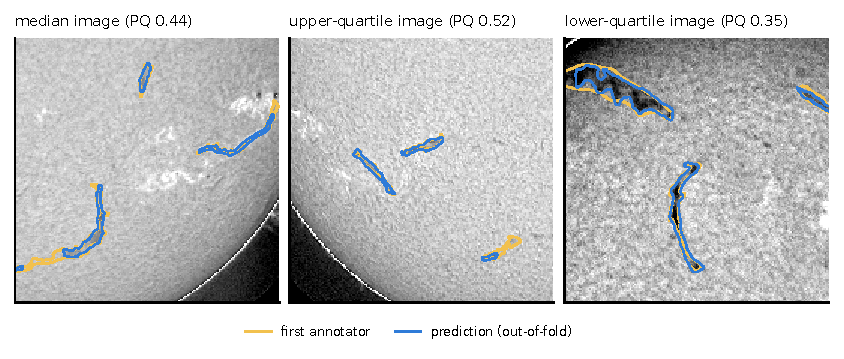
\includegraphics[width=\textwidth]{figures/fig_examples.pdf}
\caption{Out-of-fold predictions after stage 3 (blue) and the first annotator's filaments (yellow) on the training images with the median (20131016185334Ch), upper-quartile (20121108155954Bh) and lower-quartile (20120110155754Bh) image PQ. Native-resolution $768\times768$-pixel crops where the annotations are densest.}\label{fig:examples}
\end{figure*}

\begin{figure}[t]
\centering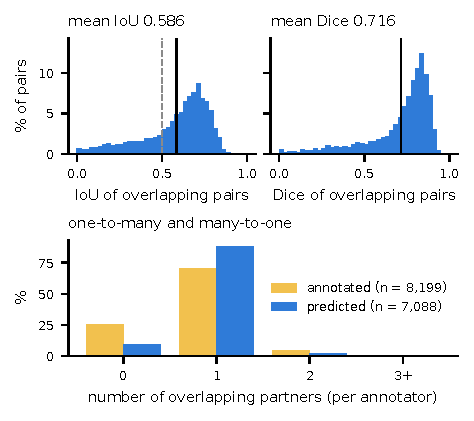
\includegraphics[width=\columnwidth]{figures/fig_diagnostics.pdf}
\caption{Organisers' diagnostics for the final out-of-fold masks: IoU and Dice of every overlapping (annotated, predicted) pair, and the number of overlapping partners per annotated filament and per prediction.}\label{fig:diag}
\end{figure}

\subsection{Where PQ is lost}
Figure~\ref{fig:gap}b classifies each annotated filament after stage 2. 59\% are matched. For 18\%, candidates touch the filament but none reaches IoU 0.5, so the candidate shapes, not the selection, limit PQ; for 12\%, a matching candidate exists but its estimated $\hat u$ (median 0.13) is below $\tau$; 6\% are touched by no candidate. Misses concentrate on small filaments (recall 0.32 for the smallest tenth, below 410 pixels) and towards the limb (0.48 at 0.70--0.85 disk radii against 0.62 near the centre). With perfect $\hat u$ the same candidates would reach PQ 0.557; this gap to the learned selection is far larger than what a finer 33-level tree adds to the bound (0.008 on two folds), so better scoring of the existing candidates is the larger lever.

\begin{figure}[t]
\centering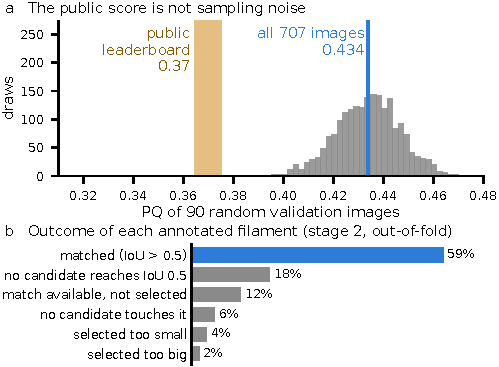
\includegraphics[width=\columnwidth]{figures/fig_gap.pdf}
\caption{(a) PQ of 2,000 random sets of 90 validation images, the size of the public test half, with the public score. (b) Outcome of every annotated filament (per annotator) after stage 2.}\label{fig:gap}
\end{figure}

\subsection{Validation and leaderboard}
Out-of-fold PQ is 0.434 (95\% interval 0.424--0.444 when resampling observation dates), while all our stage-2 and stage-3 submissions score 0.37 on the public half of the test set. We tested four explanations before trusting the validation. \emph{Sampling noise:} random sets of 90 validation images span 0.408--0.458 (Figure~\ref{fig:gap}a); 0.37 lies about five standard deviations below the mean. \emph{Input shift:} a classifier cannot separate validation candidates from test candidates (AUC 0.42--0.51; 0.57 between 2-model and 10-model maps of the same test images), and the number of selected filaments per image is the same (6.0 and 5.9). \emph{Optimistic threshold:} choosing $\tau$ on the other folds costs 0.002. \emph{Composition:} reweighting validation images to the test's site and year mix gives 0.434 and 0.431, per-annotator PQ ranges from 0.37 to 0.54 for annotators with at least 20 images, and test images are closer in time to training images than validation images are, while validation PQ does not depend on that distance. None of these explains a drop of 0.06, so we attribute it to the hidden test labels or the composition of the public half, which we cannot test, and expect the private score near 0.37 rather than 0.43.

\subsection{Negative results and reproducibility}
A finer tree (33 levels), larger or smaller LightGBM models ($-0.002$) and EfficientNet-B3 encoders (which fail on the Kaggle T4 image with a CUDA misaligned-address error in half-precision depthwise convolutions) did not help; the refiner missed its pre-set adoption threshold. The repository contains the modules (metric, candidates, scorer, selection, refinement), unit tests, the Kaggle training scripts and their logs, the fold split, and an end-to-end notebook. In reuse mode the notebook rebuilds stages 2 and 3 and the out-of-fold rows of Table~\ref{tab:results} from the published stage-1 maps on CPU in about an hour; in full mode it retrains all models (about 8 hours on two T4 GPUs). Our PQ implementation agrees with the organisers' notebook to $10^{-6}$, and their code run unmodified on our out-of-fold masks gives the same 0.4338.

\section{Acknowledgment}\label{sec:acknowledgment}
The organization of the Filament Segmentation Challenge 2026 is partially supported by the U.S. National Science Foundation (NSF) under Grant No. 2209912 and 2433781, directorate for Computer and Information Science and Engineering (CSE), and Office of Advanced Cyberinfrastructure (OAC), and Grant No. 2511630, AST Division Of Astronomical Sciences and MPS Directorate for Mathematical and Physical Sciences.

The Filament Segmentation Challenge 2026 is sponsored by the U.S. National Science Foundation (NSF) National Solar Observatory (NSO).

This work utilizes GONG data obtained by the NSO Integrated Synoptic Program, managed by the National Solar Observatory, which is operated by the Association of Universities for Research in Astronomy (AURA), Inc. under a cooperative agreement with the National Science Foundation and with contribution from the National Oceanic and Atmospheric Administration. The GONG network of instruments is hosted by the Big Bear Solar Observatory, High Altitude Observatory, Learmonth Solar Observatory, Udaipur Solar Observatory, Instituto de Astrofísica de Canarias, and Cerro Tololo Interamerican Observatory.
\bibliographystyle{ACM-Reference-Format}
\bibliography{main}
\end{document}
